% set 0.5 inch indentation
\setlength{\parindent}{0in}
% set paragraph space = 0 space
\setlength{\parskip}{1.5mm}
% set line space 1.5
\setlength{\baselineskip}{1.6em}

\chapter{INTRODUCTION}
\section{Background}
Masked Language Modeling (MLM) is a fundamental task in the training of vision-language (VL) models \cite{albef, mplug, uniter, beit-3}. 
Typically, a subset of word tokens is randomly masked at a fixed percentage during training, with the model tasked to predict the masked tokens based on information from the visual modality. 
However, \citeA{mask_object} demonstrated that many of the masked tokens are often stop-words or punctuation, which result in the model relies more heavily on language patterns that do not require visual understanding.
Thus, exploring the impact of masking strategies has become another research area for improving the effectiveness of VL models.

Some work explore the the impact of token masking strategies on multimodal model performance. 
\citeA{mask_object} introduced an object token masking strategy, where object tokens in image captions are selectively masked, and the model is pre-trained from scratch.
This approach led to superior performance compared to random masking. 
Furthermore, \citeA{selective_masking} demonstrated that selectively masking infrequent words from the pre-training dataset during continued training enhances model performance on out-of-domain datasets, highlighting the importance of domain-aware masking techniques.

However, the effects of masking strategies based on linguistic features remain under-explored. 
Thus, we design experiments to analyze the impact of selective masking based on the part-of-speech categories in image captions.

In this work, we explore the effects of masking each part-of-speech category by masking each part-of-speech of each image captions as shown in figure \ref{fig:overview}. 
As each part-of-speech contributes uniquely to the meaning of a sentence, for instance, nouns typically represent objects, while verbs describe actions, which often require contextual understanding. 
We hypothesize that masking verbs is the best way to increase the VL model understanding, as verbs in a sentence represent interactions between objects and require the model to rely more on visual information.
By selectively masking different part-of-speech, we can gain insight about how each part-of-speech category affects the alignment between vision and language modalities. 
The experiment is designed to answer the following questions:
\begin{enumerate}
    \item How does selective part-of-speech masking affect the alignment of vision and language modalities?
    \item How does part-of-speech masking change the contribution of the vision and language modalities to the model's output?
    \item How does specific masking impact the performance of vision question answering tasks, particularly in terms of improvements based on the type of question?
\end{enumerate}

\begin{figure}[h]
    \caption{Overall methodology}
    \label{fig:overview}
    Pre-training model with MLM task by masking token based on part-of-speech of the image captions.
    \begin{center}
        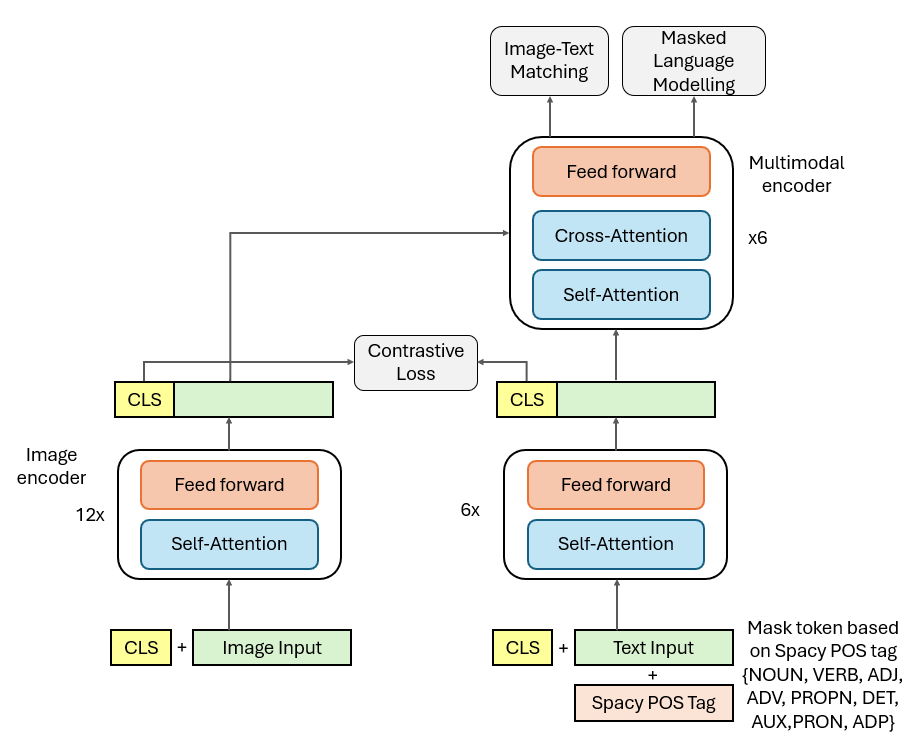
\includegraphics[width=0.6\textwidth]{Images/overview.png}
    \end{center}
    \small
\end{figure}

\section{Objective}
The objectives for our experiment are as listed.
\begin{enumerate}
    \item Pre-trained VL model for the experiment to identify the performance of masking in each part-of-speech.
    \item Benchmarking our method against specialize dataset based on linguistic feature \cite{valse} for better understanding of the masking effect.
    \item Analyze contribution from each modality of vision and language to the prediction output based on MM-Shap \cite{mm-shap}.
\end{enumerate}

\section{Scope}
\begin{enumerate}
    \item The training and testing dataset are both natural image.
    \item The model architecture is cross-attention model due to the ability of cross attention to jointly predicted answer based on another modality.
\end{enumerate}


